\chapter{Experiments and Results}\label{chapter:measurements}

This chapter delves into the empirical exploration conducted to understand the interplay between various control variables and the performance of Matrix Profiling algorithms on the Cerebras Wafer Scale Engine (WSE).

In this study, we systematically investigate the influence of four pivotal control variables: \texttt{Time Series}, \texttt{Tile Size}, \texttt{Window Size}, and \texttt{Resource Rectangle}, on the efficiency and accuracy of Matrix Profiling computations on the Cerebras WSE. By meticulously varying these parameters and analyzing their impact on computational metrics such as execution time, memory utilization, and result fidelity, we aim to unravel insights crucial for optimizing Matrix Profiling workflows on this cutting-edge hardware platform.

Within this chapter, we outline our experimental methodology, detailing the setup, execution, and analysis of Matrix Profiling experiments on the Cerebras WSE. Through rigorous empirical investigation, we endeavor to shed light on the intricate relationship between control variables and Matrix Profiling performance, ultimately contributing to the advancement of time series analysis techniques on state-of-the-art computing architectures.

Our findings hold implications for researchers and practitioners seeking to harness the potential of novel hardware platforms like the Cerebras WSE for accelerating Matrix Profiling tasks. By elucidating the optimal configurations and parameters for Matrix Profiling experiments, we aim to facilitate the development of scalable, high-performance solutions tailored to the demands of modern data analysis workflows.

\clearpage

\section{Model}

In this chapter, we delve into a series of experiments aimed at elucidating the impact of various control variables on the performance and efficiency of Matrix Profiling algorithms executed on the Cerebras Wafer Scale Engine (WSE). These experiments are guided by the following control variables:

\begin{itemize}
    \item \textbf{Time Series (\textit{s})}: The length and complexity of the time series data under analysis.
    \item \textbf{Tile Size (\textit{t\_s})}: The size of the Tile allocated to a single PE, which directly influences the parallelism and computational efficiency.
    \item \textbf{Window Size (\textit{m})}: The size of the sliding window used for local pattern discovery within the time series data.
    \item \textbf{Resource Rectangle (\textit{r\_r})}: The configuration of resources allocated within the Cerebras WSE for executing the Matrix Profiling algorithm.
\end{itemize}

These control variables serve as the foundation for our experimental design, allowing us to systematically explore their implications on the overall execution and efficiency of the Matrix Profiling algorithm on the Cerebras WSE.

The Matrix Profiling algorithm exhibits a time complexity of \(O(n^2)\), where \(n\) represents the length of the time series data. This runtime complexity is directly influenced by the \texttt{Tile Size} parameter, as it dictates the granularity of computation performed by individual PEs within the Cerebras WSE.

Our experimental design implicitly assumes a one-to-one mapping between the number of tiles in the given time series data and the number of PEs allocated on the Cerebras WSE. This constraint arises from the memory limitations of individual PEs and the lack of support for streaming data in and out of the fabric within the Cerebras architecture.

Each of the following experiments introduces the theoretical model for the experiments first and the conclusions derived from them, and then the empherical results from the simulator and the hardware. The simulator provides only the number of cycles spent on each individual PE and we derive measurements from the same.

\begin{itemize}
    \item Insert Simulator Hardware parameters here. 
\end{itemize}
The Hardware experiemnts were run on the 
\begin{itemize}
    \item Insert Hardware execution parameters here.
\end{itemize}

\section{Execution Time}

The following section looks into the Execution time for the main kernel and overall execution on the Cerebras WSE-2.

To determine the runtime of the kernel, the CSL language exposes hardware clock cycle timer data that can be queried and saved over the runtime of a kernel and reported back to the host. The total wall time of a kernel can be computed by determining the maximum number of cycles used by any PE during the kernel and dividing it by the clock rate of the WSE-2 (850 MHz). While some degree of thermal throttling will occur, the WSE-2 implements
throttling by injecting “nop” commands rather than by adjusting the clock speed
itself, such that any thermal “nop” cycles are included when measuring kernel cycle
counts. This method of measuring kernel runtime performance by recording clock
cycles is used throughout this paper whenever runtime data is reported and is the
standard method for recording performance data on Cerebras machines \cite{9}

\subsection{Kernel Execution Time}
The algorithm to compute the Matrix profile as defined in Section 3.4, is an \(O(n^2)\) algorithm and hence, the execution time is directly propotional to the tile size. We gradually increased the tile size ($t_s$) across the experiment and keeping all the other parameters constant. Since the \textit{Distance Matrix} needs to be decomposed into smaller or larger tiles, this has a implication on the size of \texttt{Resource Rectangle}





\begin{figure}[h!]
    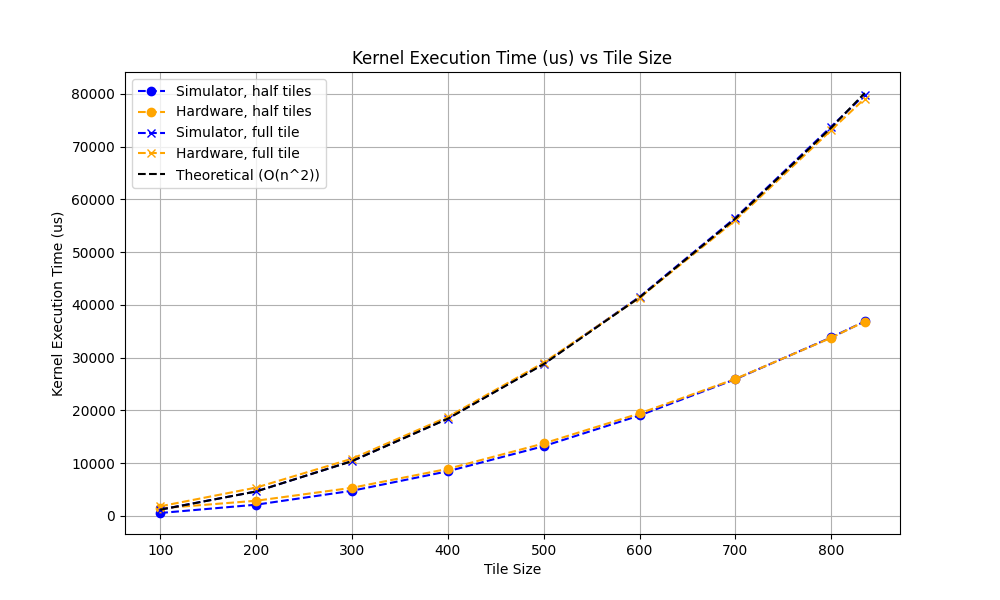
\includegraphics[scale=0.5]{execution_6}
    \centering
    \caption{Plot of Observed Execution time of different tile sizes on the Simulator}
\end{figure}

\subsubsection{Floating point operations per second}

With the empherical values obtained from the simulator, 
\begin{equation*}
    \text{FLOPs} = 2 \times \left( 6 \times (t\_s \times t\_s) +  2 \times m + 7 \times t\_s\right)
\end{equation*}

\begin{figure}[h!]
    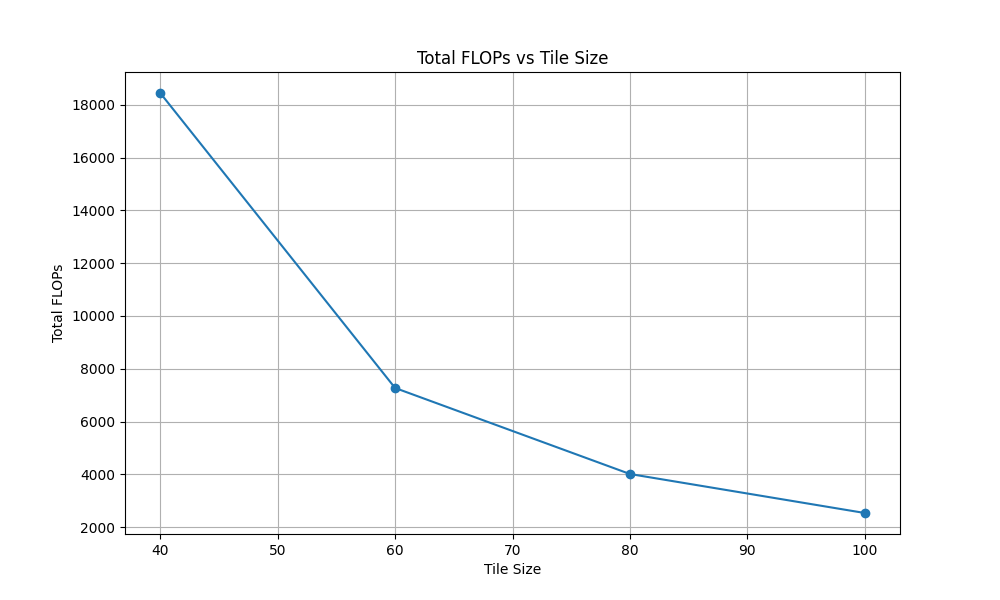
\includegraphics[scale=0.5]{flops.png}
    \centering
    \caption{Floating point operations vs tile size}
\end{figure}

\subsection{Overall Execution time}

To look at the performance of the entire program and not just at the kernel execution time, we focused on small to larger datasets of $s = 1000 \dots 100000$.

The following experiments are conducted with a random walk time series of varying sizes ($s$), a constant tile size ($t\_s$) of 100 a constant window size ($m$) of 6.
The increasing Time series sizes were chosen to capture the impact of memory transfers and kernel execution on larger datasets since it transmits a increasingly more data and computes on a greater \texttt{Resource Rectangle}. We reached a 

    
\section{Memory}

Matrix profiling is an memory intensive algorithm since it involves a lot of prefactors in the computation, The Cerebras SDK does not expose any metrics on Memory consumption, Hence, we present our mathematical model on memory usage on a single PE and compare it to what was practically possible. In order to arrive at a model of memory consumption for a single tile, we need to look at the variables involved in the computation of a single tile of size $s$ and for a window of size $m$. therefore,
\begin{equation}
    M = F\left(MP_a, MPI_a, MP_b, MPI_b,T_a, T_b, inf, df, dg, args\right);
\end{equation}

\[
\begin{array}{c}
    M = sizeof(2 * (s + m) + 10 * (s - m + 1) + 7)\\
    M = (12 * s - 8 * m + 17) * 32 / 8 / 1024\\
\end{array}
\]

\begin{figure}[h!]
    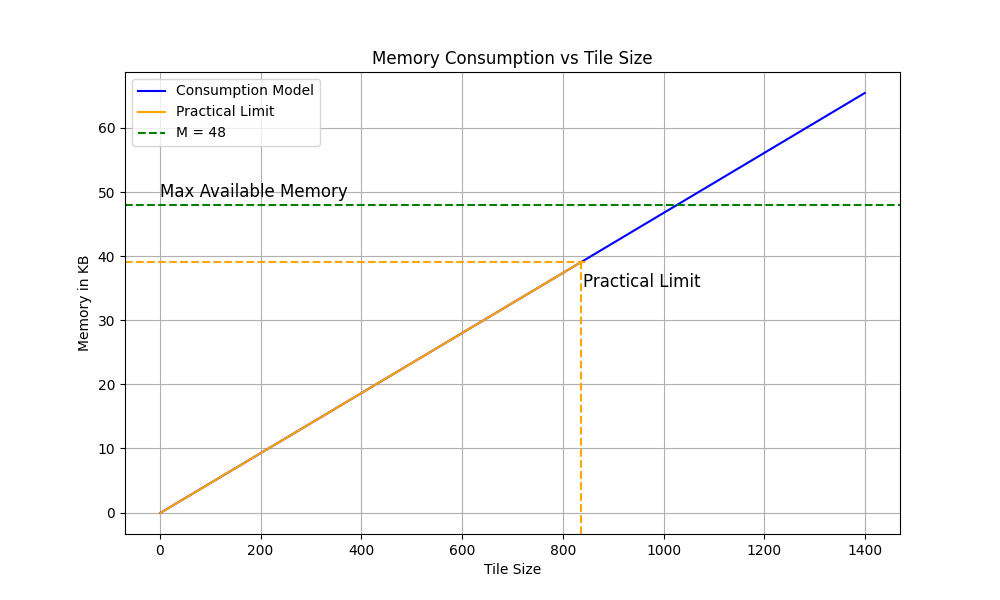
\includegraphics[scale=0.5]{memory_6}
    \centering
    \caption{Memory Usage of a single PE plotted against Tile Size. The theoretical limit to the tile size is 1010 but what is observed is a maximum limit of 100 per PE. Practically, we were able to use only 4.566 KB of memory of the PE.}
\end{figure}

We reaching a practical limit of 4.566 KB. We encountered compilation issues on the Cerebras compiler that did not allow us to allocate larger arrays and led to a stack size issue. Sadly, we couldn't further investigate into the reason behind it due



\section{Weak Scaling Experiments}

Since the Cerebras WSE-2 is primarily focused on weak scaling, We look at the possible implications of Weak Scaling on the device using various configuration and analyse the implication on memory transfer speeds and execution time. We begin our weak scaling study by fixing the window size and tile size, $m$ and $t\_s$ to 100 and 6 respectively and increase the time series size gradually. We choose to use to random walk algorithm to generate our time series.
The sensitivity in performance to $s$ is also investigated. We choose to create \texttt{Resource Rectangles} of different sizes to study the impact varous resource allocation schemes on the execution time of the algorithm.

We expect linear growth in the total throughput of the kernel

\section{Precision Evaluation}

Given the unpredictable nature of real-world data, which often includes numerous constant areas, numerical instability arises as a concern. The similarity of z-normalized subsequences is of particular interest to many researchers. In constant regions, the standard deviation is zero. Additionally, near-constant subsequences pose challenges as they may pass a bit-level test for two distinct values, yet result in division by a number nearly approaching zero.

In this section, we take a look at the impact of Cerebras lower precision floating point limitation. We compare the error study provided by SCAMP on single precision \cite{4} to simulated random time series on different distribution.
Since Cerebras works only with reduced floating point precision values, It leads to a loss of information in the MP when compared to a double precision algorithm. Although the difference is subtle, it is noticable on larger data sets.
\clearpage
\begin{table}[h!]
    \centering
    \caption{Maximum absolute error (Pearson Correlation) for various datasets on SCAMP in single precision. \cite{4}\\}
    \begin{tabular}{c c c c} 
     \hline
     Maximum Absolute Error & Size (m) & SCAMP SP \\ [0.5ex] 
     \hline
     Whitefly & 2.5M (1000) & $3.75^*10^{-2}$ \\ [1ex]
     \hline
     ECG & 8.4M (100) & $3.14^*10^{-4}$ \\ [1ex] 
     \hline
     Earthquake & 1.7M (200) & $6.35^*10^{-1}$ \\ [1ex] 
     \hline
     Power Demand & 10M (4000) & $4.85^*10^{-2}$ \\ [1ex] 
     \hline
     Chicken & 9M (1000) & $4.92^*10^{-2}$ \\ [1ex] 
     \hline
    \end{tabular}
\end{table}

These results are comparitive to the double precision version of SCAMP, hence, the results are very similar. Since we did not have the compute power to execute such large datasets, we setup an simpler experiment involving different random distributions as shown in Figure 5.3. Although this does not provide a simulation of real life dataset, we wanted to look at anomolies in error rates across different distributions.

\begin{figure}[h!]
    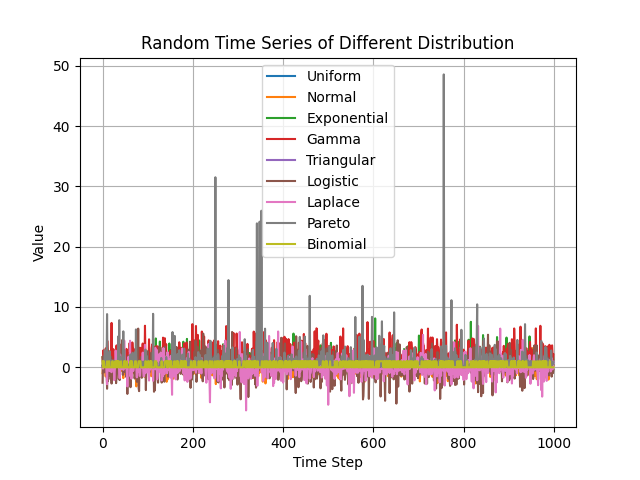
\includegraphics[scale=0.5]{random_distribution_for_error}
    \centering
    \caption{Time series of different random distributions}
\end{figure}


\begin{figure}[h!]
    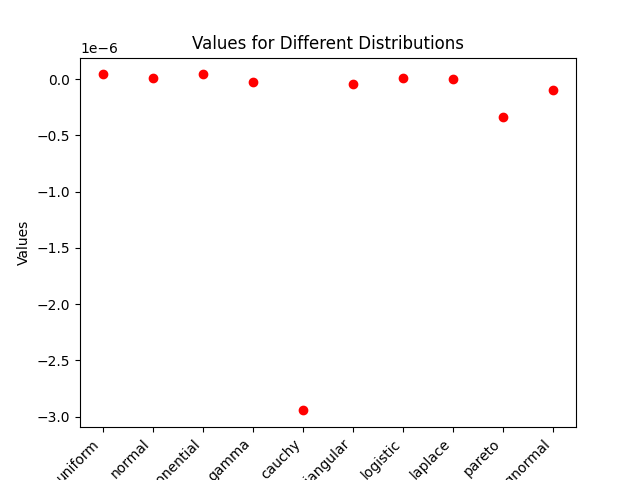
\includegraphics[scale=0.5]{distribution_values_scatter_plot}
    \centering
    \caption{Error rate on different probabilistic distributions}
\end{figure}

\section{Comparison to CPU \& GPU Baseline}

Now that we have enough experimental results from the Hardware and Simulator, We can compare the performance of the Cerebras WSE-2 with traditional GPUs. In Table 4.1, we take a look at the SCAMP performance on random walk datasets of various lengths \cite{4} and compare them to the runtime of similar random walk time series on the Cerebras WSE-2 simulator on a fabric of size $w$ = 500 and $h$ = 500 executed using iterative scheduling.


\begin{table}[h!]
    \centering
    \renewcommand{\arraystretch}{1.25} % Adjust the spacing between rows
    \caption{Scamp Runtime}
    \begin{tabular}{|| c | c | c | c ||} 
        \hline
        Implementation & \multicolumn{2}{c||}{SCAMP-GPU} & Cerebras WSE-2 \\ [0.5ex] 
        \hline
        Architecture & V100 & V100 & \\
        \hline
        Precision & DP & SP & SP \\
        \hline\hline
        $2^{18}$ & 0.28s & 0.24s & \\
        \hline
        $2^{19}$ & 0.68s & 0.57s & \\
        \hline
        $2^{20}$ & 2.05s & 1.42s & \\
        \hline
        $2^{21}$ & 6.99s & 4.38s & \\
        \hline
        $2^{22}$ & 25.8s & 15.5s & \\
        \hline
        $2^{23}$ & 96.8s & 52.5s & \\
        \hline
    \end{tabular}
\end{table}



\section{Execution on Real world datasets}

\begin{center}
    \begin{tabular}{c c c c c c} 
     \hline
     Time series & n & m & Max & Min & Up.\% \\ [0.5ex] 
     \hline
     5 & 88 & 788 & 6344 \\ [1ex] 
     \hline
    \end{tabular}
\end{center}

We used a diverse set of time series for the experimental evaluation,
whose parameters are shown in Table 1. We can see the number of
samples, \textit{n}, and the window size or subsequence length, \textit{m}, used for
each series, as well as the maximum and minimum values. The name of
each series is descriptive of the type of content they contain. Note that
all time series used in this work come from real data [33]. The last rows
of the table identify the series used to evaluate the proposals with large
data sets, including an extra-large one of nearly 11M samples [18]. The
last column shows the percentage of all profile update attempts that
indeed write the matrix profile and matrix profile index arrays, using
the baseline SCAMP algorithm with one thread; i.e., the if statements in
Lines 4, 4, 4 and 4 in Fig. 4 which become true.